\pdfminorversion=4
\documentclass[mathserif,xcolor={dvipsnames,table}]{beamer}
\mode<presentation>{\usetheme{Warsaw}\usecolortheme{crane}}
\usepackage{centernot}
\usepackage{graphicx}
\usepackage{geometry}
\usepackage{tikz}
\usetikzlibrary{shadows}
\usepackage{hyperref}
\usepackage[utf8]{inputenc}
\usepackage[english]{babel}
\usepackage[T1]{fontenc}
\usepackage{lmodern}
\usepackage[babel=true]{microtype}
\usepackage{amsmath}
\beamertemplatenavigationsymbolsempty

\title{\textbf{Not Sucking in the UNIX Environment}}
\date{}
\author{CS4803UWS at the\\
Georgia Institute of Technology
}

\begin{document}

\begin{frame}
\titlepage
\begin{center}

\includegraphics[scale=0.33]{images/uws.png}\\
\vspace{.1in}
\tiny{copyright \copyright\ 2013}\\

\includegraphics[scale=.25]{images/cc-logo.pdf}

\includegraphics[scale=.25]{images/cc-new.pdf}

\includegraphics[scale=.25]{images/cc-share.pdf}\\
\tiny{creative commons 3.0 share-alike attribution license}
\end{center}
\end{frame}

\begin{frame}{Perl}
Please don't write perl.
\end{frame}

\begin{frame}{Shell scripts}
\begin{itemize}
\item POSIX conformance: probably not worth it
\item First line: \texttt{\#!/bin/sh} or \texttt{/usr/bin/env} \textit{shell}
\item Second line: \texttt{set -e || exit 1}
\item Pipelines only fail if the last command fails\footnote{Unless \texttt{-o pipefail} (bash-only) is used.}
\item Catch subshell errors via assignment
\item \texttt{trap} on signals and pseudo-signal 0\footnote{bash allows \texttt{trap}ping EXIT as a synonym for 0.}
\end{itemize}
\end{frame}

\begin{frame}{Redirection}
\begin{itemize}
\item Redirect to stderr: \texttt{>\&2}
\item Functions can be redirected at definition, \textit{and} at invocation
\item Pipes can't target functions (use \texttt{read} if you must)
\item Redirect both stdout and stderr: \texttt{>} \textit{redir} \texttt{2>\&1}
\item Send stderr to stdin through pipe: \texttt{|\&} (\texttt{2>\&1 |})
\item Duplicate to stdout and a file: \texttt{| tee} \textit{file}
\item Append: \texttt{>}\texttt{>}\textit{file}\hfill Dup and append: \texttt{| tee -a} \textit{file}
\item \texttt{/dev/std\{in, out, err\}}: stdio in a filename context
\end{itemize}
\end{frame}

\begin{frame}{GNU Autotools in one terrible diagram}
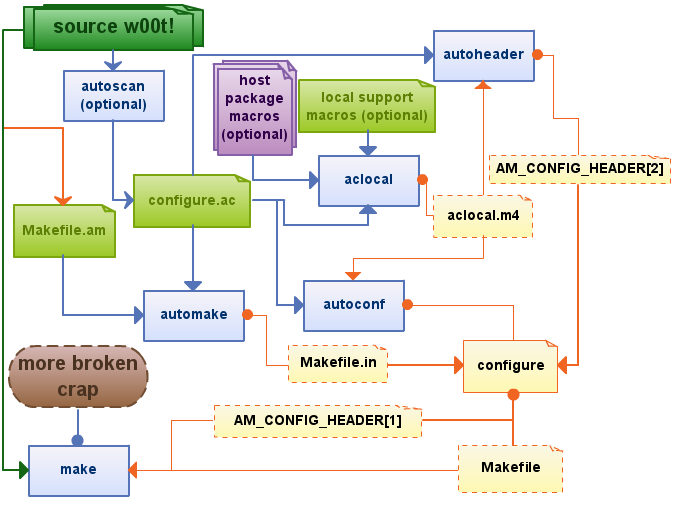
\includegraphics[scale=0.45]{images/circleoflife.png}
\end{frame}

\begin{frame}{FIXME}
\huge FIXME approximately 10 more pages...
\end{frame}

\begin{frame}{Recommended reading}
\begin{itemize}
\small{
\item Dennis Ritchie. ``Evolution of the Unix Time-sharing System'' (1979).
\item Neil Brown. ``Ghosts of UNIX Past'' LWN, in four parts (2004).
\item Tom Christiansen. ``\texttt{csh} Programming Considered Harmful'' (1995).
\item Mendel Cooper. ``Advanced Bash-Scripting Guide'' (2012).
\item Peter Krumins. ``\texttt{sed} One-Liners Explained'' (2008).
\item Peter Krumins. ``\texttt{awk} One-Liners Explained'' (2008).
\item Steve Yegge. ``Ancient Languages: Perl'' (2004-12-04).
\item Neal Stephenson. \textit{In the Beginning was the Command Line} (1999).
}
\end{itemize}
\end{frame}

\begin{frame}{Hack on!}
``One of the main causes of the fall of the Roman Empire was that, lacking zero, they had no way to indicate successful termination of their C programs.''\hfill---Robert Firth
\vfill
``It's easier to port a shell than a shell script.''\hfill---Larry Wall
\end{frame}

\usebackgroundtemplate{%
\vbox to \paperheight{\hbox to \paperwidth{\includegraphics[scale=0.61]{images/gt.jpeg}}}}
\begin{frame}
\end{frame}

\end{document}
